\subsection{Removing Schottky Effects to find $I_o$}

We first wish to look at the relationship between the Anode current ($I_a$) and the Anode's Voltage ($V_a$). This is in part to verify the Schottky Effects, and in an effort to obtain estimates for the Anode Current without electrical field from these fits using Equation \ref{plot_1eqn} by comparing $\ln(I_a)$ with $\sqrt{V_a}$. We know that all other terms should be constant since our vacuum tube states that "The guard rings ensure continuous and homogeneous anode-cathode field and eliminates 'fringe' effects." \cite{GRD7}. The temperature is the only other quantity which may change, but it will not per trial as the filament current is monitored during the runs and as we will later see is an empirically known quantity through use of Equation \ref{temp} in relation to the filament current.

\par

We also note at this time that the presented $V_a$ is a calculated correction on our $V_a$, which is calculated by taking the known anode voltage and subtracting off the midpoint of the filament voltage as we can see is necessary from our Circuit Diagram (Figure \ref{Circuit}) \cite{LabProcedure}. We completed the analysis with and without correction and this made no difference to final results as this effect applies to each voltage and any changes are dominated by an anode voltage which are 2 orders of magnitude larger

\begin{figure}[ht!]
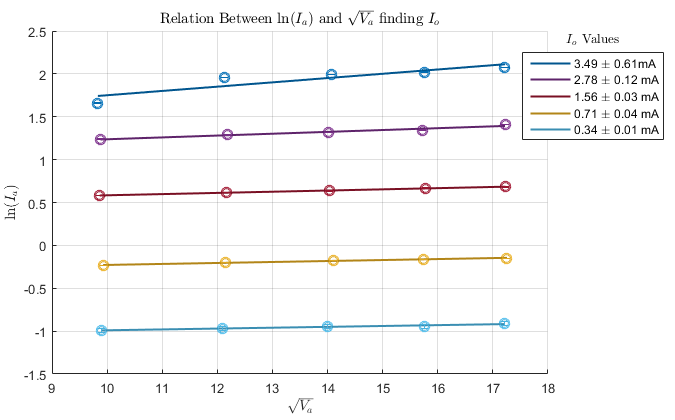
\includegraphics[scale=.95]{figures/plot_1_Io.png}%
\caption{The plots of anode current and voltage to find values for the anode current without effects of an electric field }%
\label{fig:plot_1}
\end{figure}

We present our $I_o$ values in  Table \ref{tab:Io_vals} which are calculated through a linear regression through using the least squares method. Intersection error estimates are provided by analyzing the standard error of coefficient estimates and scaling them to the final $I_o$ values. 

From this analysis it can be seen see that the Schottky Effects appear to be modelled well by the modified Richard-Dushman Equation as the plots of based around linearizing our Schottky modified Richard-Dushman Equation (Equation \ref{plot_1eqn})create a linear fit which has a high accuracy of prediction (goodness of fit ($R^2$) is greater than .95 and percentage error is less than 5\%) for all of the fits other than the highest anode current.
\begin{table}[h]

  \footnotesize{
            \begin{tabular}{llll}
            \hline
            $I_a $ (mA) & \multicolumn{2}{l}{\makecell{$I_o$ (mA)}}& $R^2$       \\ \hline
            8.00     & 3.49  & $\pm$ .61            & 0.818     \\
            4.00     & 2.78  & $\pm$ .12            & 0.955     \\
            2.00     & 1.56  & $\pm$ .03            & 0.996    \\
            0.80     & 0.71  & $\pm$ .04            & 0.967  \\
            0.40     & 0.34  & $\pm$ .01            & 0.951  \\\hline
            &&&\\
    \end{tabular}
        
    }
\caption{The values of $I_o$ which are derived from the linear fits. Also included are error estimates and goodness of fit statistics.}%
\label{tab:Io_vals}
\end{table}

This run with the highest anode current appears has much less predictive power, with a low $R^2$ value of .818 and a high percentage error of 17.46 \%. We note that if the lowest voltage value is exclueded, then the $R^2$ value increases to .964 and the percentage error decreases to 3.16\%. This indicates this point may be an outlier. However, two other sets of data were taken which both show the same relation as is seen in Figure \ref{fig:plot_1}. This leads to us to the conclusion that this non-linearity appears to be physical. However the origin of this non-uniformity is unclear. It is possible that a reaction creates a film on the filament which changes the work function of the filament for the first couple of data points, but this seems unlikely due to the vacuum containing an inert gas to minimize this effect and large warm-up times were allowed to allow for surface films to dissipate.
 \par
 
\subsection{Finding $w_o$ through the Richard-Dushman Equation}

Our second graph is a relation based on liearizing the Richard-Dushman equation as presented in Equation \ref{plot_2eqn}. This relation is based upon temperature, but we note that this is not a directly measured quantity in our experiment. But we will present an empirically known relation of filament current ($I_f$) with the filament diameter to find the temperature in Equation \ref{temp} \cite{LabProcedure} We also note the filament diameter is a given quantity with some differences in value depending on documentation source. \cite{LabProcedure} \cite{GRD7}. Since it is unknown how inaccurate the temperature is, we have not attempted to estimate error. We will also note that it is assumed in the derivation that the temperature is constant across the voltage ramp, which is untrue, but the current was monitored and the deviations appeared to be on the order of $< 1\%$ hence this error has not been included in further discussions. 

\begin{align}
    T = 60.2 \sqrt{B(1 + \num{83e-6} B )}, B = \left. I_f \middle /d^{\sfrac{3}{2}} \right. \label{temp}
\end{align}

\begin{figure}[ht!]
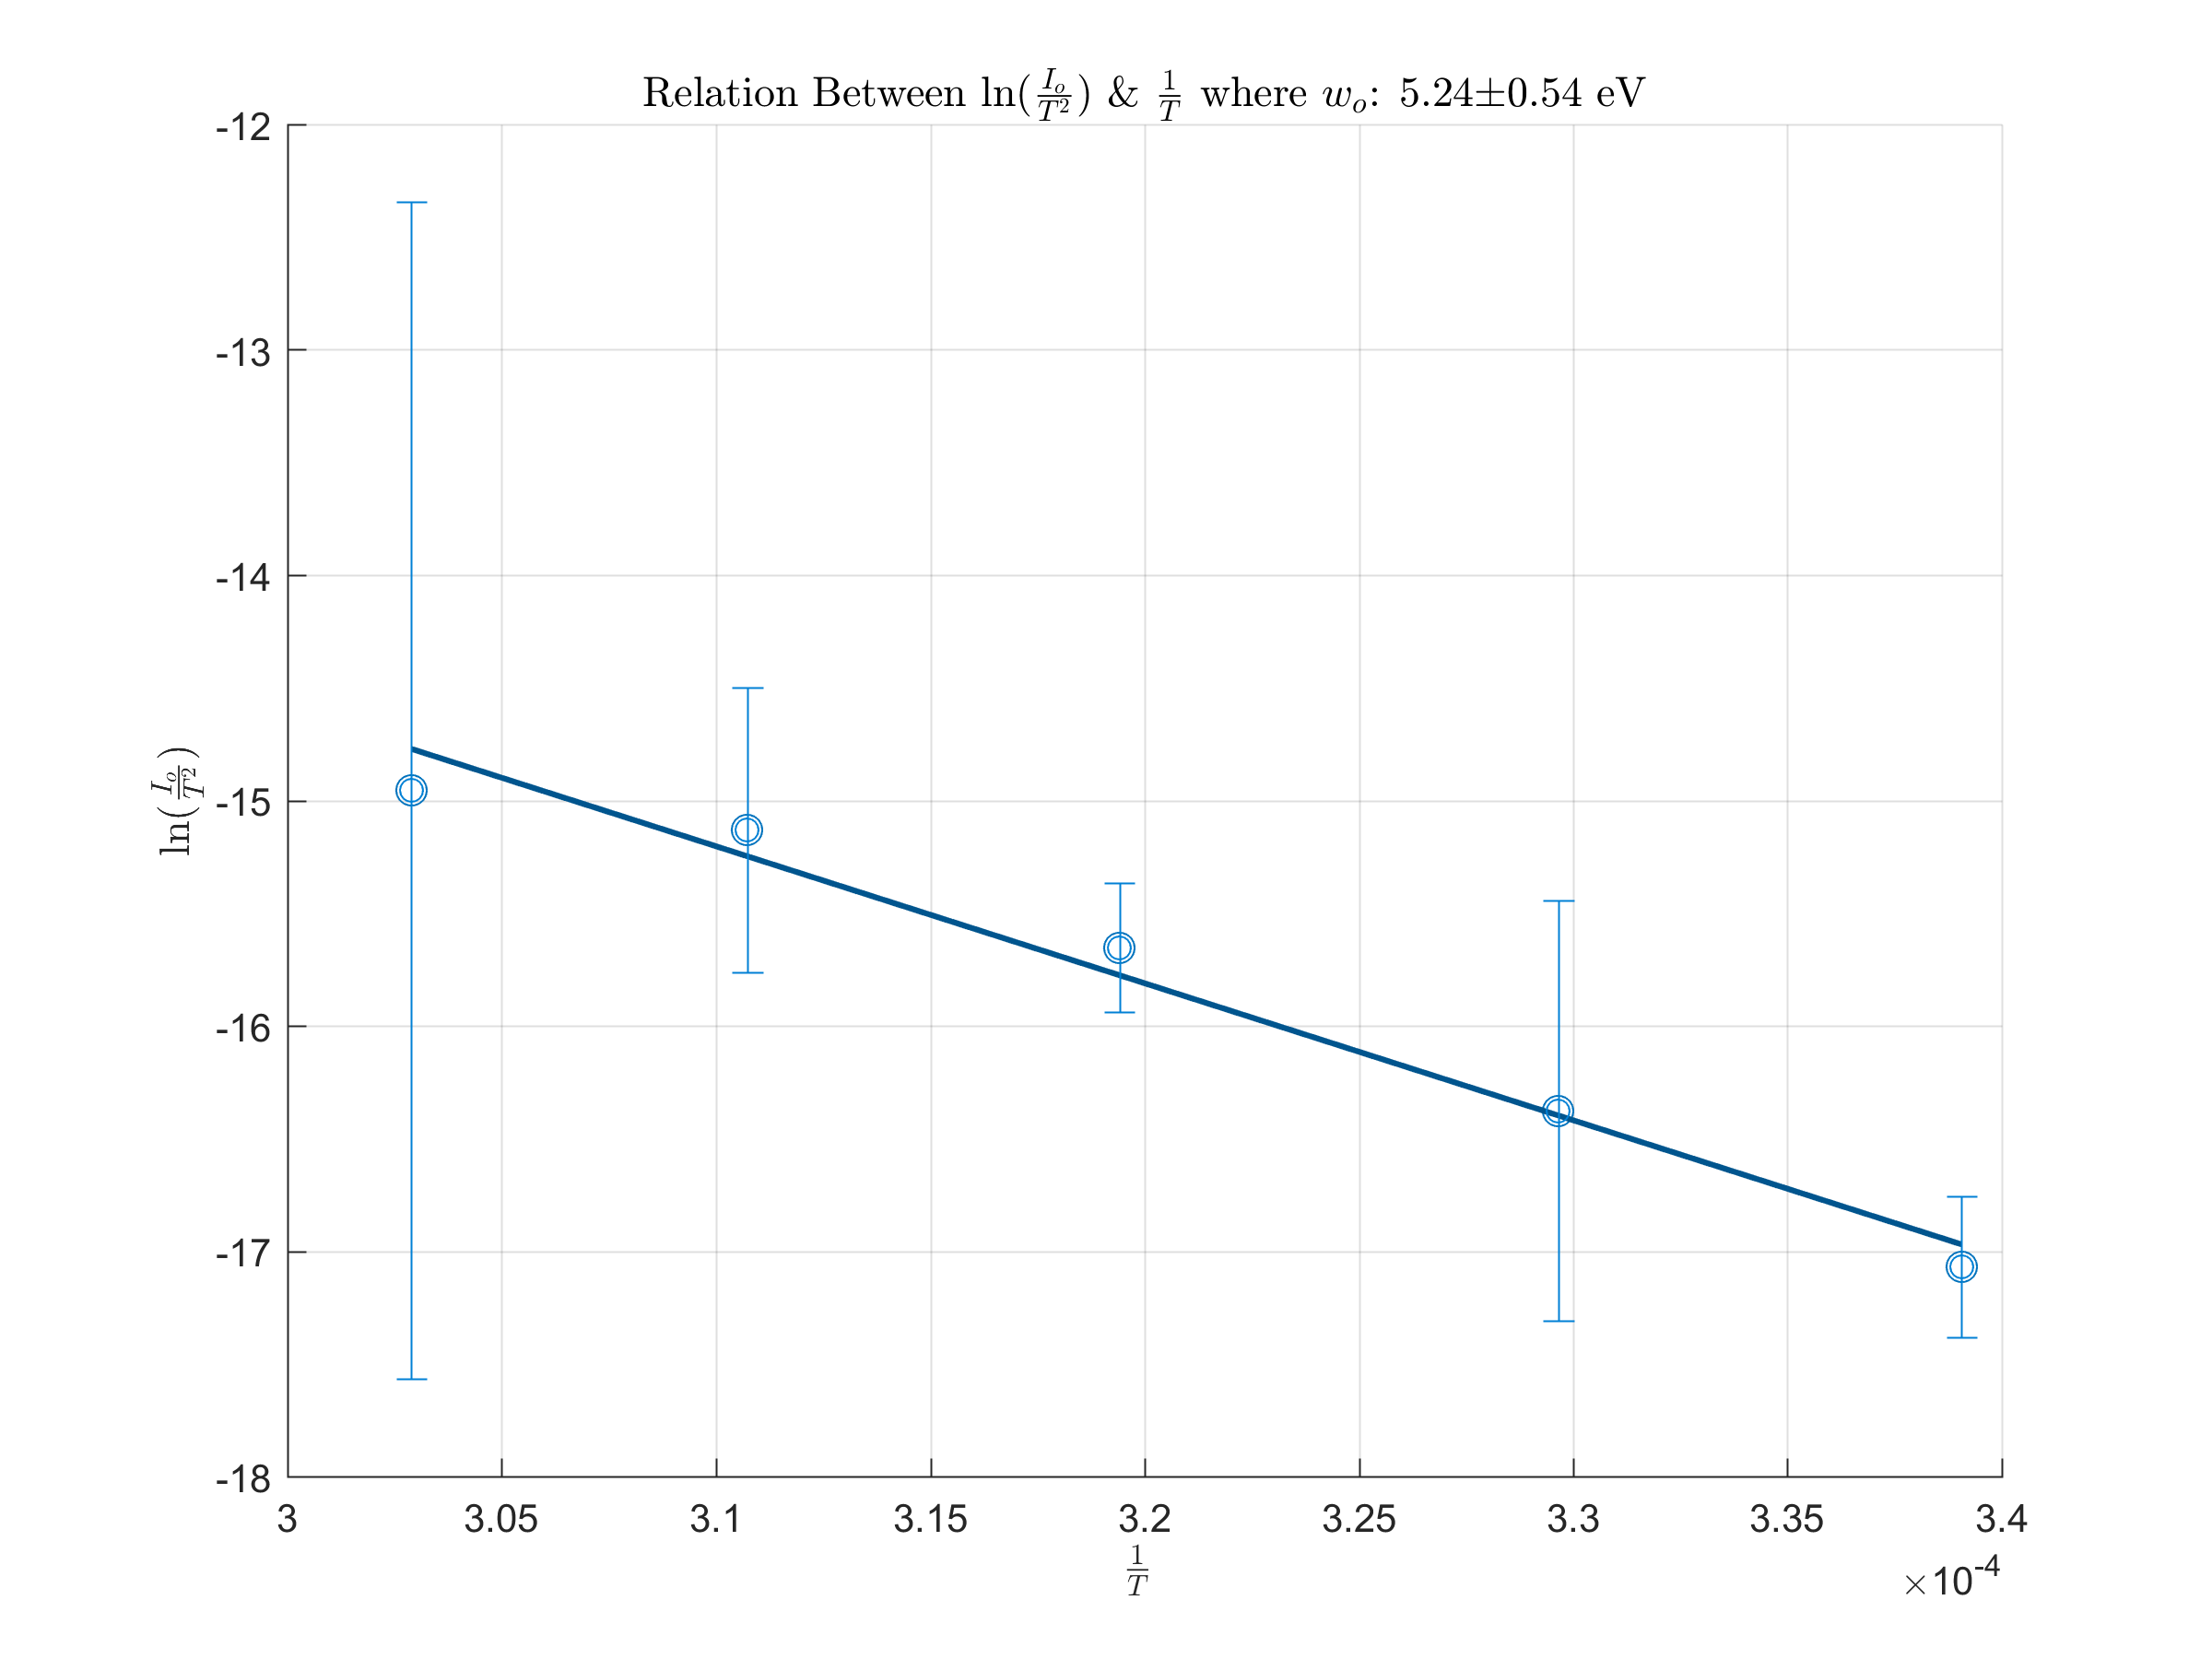
\includegraphics[scale=.8]{figures/plot_2wo.png}%
\caption{The plots of initial current scaled with temperature give us a relation for the work function }%
\label{fig:plot_2}
\end{figure}

We see that we are able to achieve a relation with high levels of linearity as well in Figure \ref{fig:plot_2}, with a high level of linearity, due to the fact that the giving us a goodness of fit of 0.977.  This indicates that the  Richard-Dushman equation holds well for this tube. However the calculated value of $w_o$ which is 5.24 $\pm$ .54 eV does not agree with the accepted work function of tungsten which is 4.5 eV in literature. Our fitting error of 10\%, does not explain the deviation from the accepted value. We believe that this deviation is caused by the unknown nature of temperature in this fit, there is no way to verify the quality of the empirically known temperature equation or the given wire diameter. Either of these issues may have caused systematic errors which are unaccounted for in our calculation of the $w_o$'s and its error.
